\documentclass{article}
\usepackage[margin=1in]{geometry}
\usepackage{amsmath,amsthm,amssymb}
\usepackage{bbm,enumerate,mathtools}
\usepackage{tikz,pgfplots}
\usepackage{chessboard}
\usepackage[hidelinks]{hyperref}
\usepackage{multicol} % Problem 35

\newenvironment{question}{\begin{trivlist}\item[\textbf{Question.}]}{\end{trivlist}}
\newenvironment{note}{\begin{trivlist}\item[\textbf{Note.}]}{\end{trivlist}}
\newenvironment{references}{\begin{trivlist}\item[\textbf{References.}]}{\end{trivlist}}
\newenvironment{related}{\begin{trivlist}\item[\textbf{Related.}]\end{trivlist}\begin{enumerate}}{\end{enumerate}}


\begin{document}
\rating{3}{3}
  Consider the intersection of a regular $n$-gon with a regular $m$-gon, both
  with sides of unit length.

\begin{figure}[ht!]
  \centering
  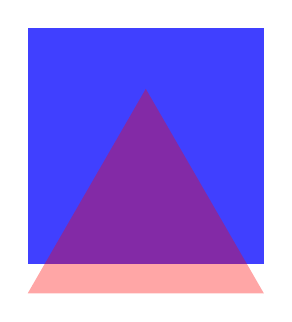
\begin{tikzpicture}[scale = 3.0]
    \fill[opacity=0.75, ultra thick, blue] (0,0) rectangle (1,1);
    \fill[opacity=0.35, ultra thick, red] (0,-1/8)--(1/2, {sqrt(3)/2-1/8})--(1,-1/8)--cycle;
  \end{tikzpicture}
  ~~~
  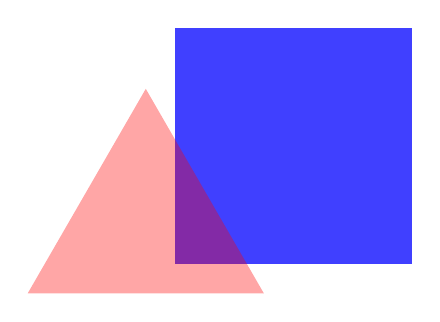
\begin{tikzpicture}[scale = 3.0]
    \fill[opacity=0.75, ultra thick, blue] (0,0) rectangle (1,1);
    \fill[opacity=0.35, ultra thick, red] (-5/8,-1/8)--(-1/8, {sqrt(3)/2-1/8})--(3/8,-1/8)--cycle;
  \end{tikzpicture}
  ~~~
  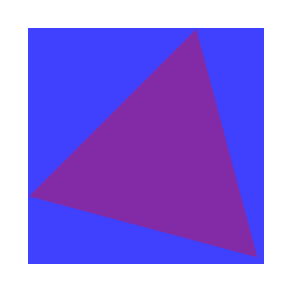
\begin{tikzpicture}[scale = 3.0]
    \fill[opacity=0.75, ultra thick, blue] (0,0) rectangle (1,1);
    \fill[opacity=0.35, ultra thick, red] (0.0063711037, 0.2863711037)--(0.713628, 0.993628)--({0.36 + sqrt(3)/2/sqrt(2)},{0.64 - sqrt(3)/2/sqrt(2)})--cycle;
  \end{tikzpicture}
  \\~\\
  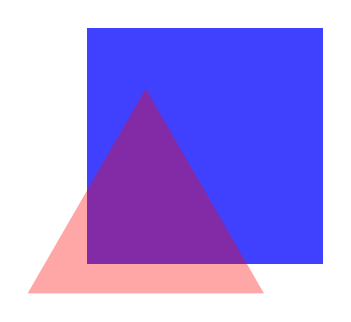
\begin{tikzpicture}[scale = 3.0]
    \fill[opacity=0.75, ultra thick, blue] (0,0) rectangle (1,1);
    \fill[opacity=0.35, ultra thick, red] (-1/4,-1/8)--(1/4, {sqrt(3)/2-1/8})--(3/4,-1/8)--cycle;
  \end{tikzpicture}
  ~~~
  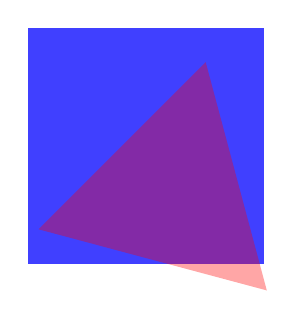
\begin{tikzpicture}[scale = 3.0]
    \fill[opacity=0.75, ultra thick, blue] (0,0) rectangle (1,1);
    \fill[opacity=0.35, ultra thick, red] (0.0463711037, 0.1463711037)--(0.753628, 0.853628)--({0.4 + sqrt(3)/2/sqrt(2)},{0.5 - sqrt(3)/2/sqrt(2)})--cycle;
  \end{tikzpicture}
  \\~\\
  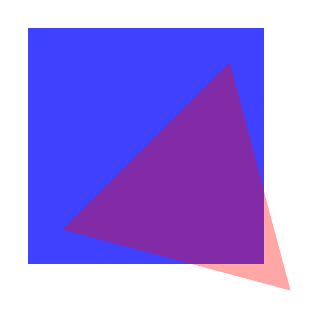
\begin{tikzpicture}[scale = 3.0]
    \fill[opacity=0.75, ultra thick, blue] (0,0) rectangle (1,1);
    \fill[opacity=0.35, ultra thick, red] (0.1463711037, 0.1463711037)--(0.853628, 0.853628)--({0.5 + +0.6123},{0.5 - 0.6123})--cycle;
  \end{tikzpicture}
  ~~~
  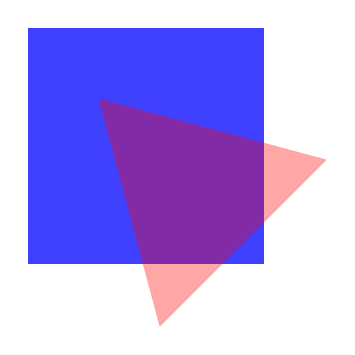
\begin{tikzpicture}[scale = 3.0]
    \fill[opacity=0.75, ultra thick, blue] (0,0) rectangle (1,1);
    \fill[opacity=0.35, ultra thick, red] (0.3, 0.7)--(0.3+0.6123+0.3535, 0.7-0.6123+0.3535)--(0.3+0.6123-0.3535, 0.7-0.6123-0.3535)--cycle;
  \end{tikzpicture}
  \caption{
    Seven (all?) classes of intersections between a $4$-gon and a $3$-gon. The
    three triangular intersections may be considered distinct because one has
    all three of its sides contributed from the triangle,
    one has two sides from the triangle, and
    one has two sides from the square.
  }
\end{figure}

\begin{question}
  What are the possible classes of polygons that can be realized as the
  intersection of an $n$-gon and an $m$-gon?
\end{question}

\begin{related}
  \item What is the largest $k$ for which a regular unit $n$-gon and $m$-gon
    can intersect in a $k$-gon?
  \item What if the polygons have unit area instead of unit length?
  \item What if the regular polygons can be any size at all?
  \item What if the polygons do not need to be regular? If the intersection does
    not need to be connected?
  \item What if the polygons have integer vertices and minimal area?
\end{related}

\end{document}
